\section{The HPRC release 2 implicit pangenome}
\label{sec:release}

The Human Pangenome Reference Consortium release 2 (HPRC r2) also provides the alignments behind its PGGB graph through impg \citep{HPRC2026resources,Garrison2024pggb}.
% src: phase1/web/hpp_readme.md:151 (HPRC2026resources): "that same all-vs-all alignment is also provided through IMPG (implicit pangenome)"
The release README calls these alignments all-vs-all, although they do not cover every haplotype pair.
% src: phase1/web/hpp_readme.md:149, 151 ("all-vs-all alignment"); scripts/fig2_release.py stdout "ordered pairs 25221 of 216690 = 11.6392%", "unordered pairs 23738 of 108345 = 21.9096%"
\authornote{Disclose who produced the HPRC r2 IMPG files. The release README (lines 149 to 191) names no producer (plan.md question Q4).}
The release ships one tracepoint (TPA) file per target haplotype, 466 files in total \citep{Kaushan2026tracepoints,Guarracino2026tpa}.
% src: phase1/web/hpp_readme.md:183 "one file per haplotype, 466 total"; data/s3_tpas.xml KeyCount 466; per target: GRCh38 TPA and per-target PAF both hold 8,916,633 records (plan.md section 4, proposal-nm-brief.md section 2)
The 466 files hold 389,234,668 alignment records in 25,070,431,026 bytes (Table~\ref{tab:datasets}).
% src: scripts/fig2_release.py stdout "files 466 bytes 25070431026 records 389234668" (bytes from data/s3_tpas.xml, records from the TPA headers in data/strtab)
They comprise 460 HPRC r2 haplotype files from 230 samples, plus GRCh38 and CHM13.
% src: scripts/fig2_release.py stdout "composition {'reference': 2, 'hprc_r2': 460, 'genbank': 2, 'hg002': 2} hprc_r2 samples 230"; stems in data/partners.tsv column 1 (hprc_r2: 104 hap1, 104 hap2, 126 mat, 126 pat)
The other four files hold the maternal and paternal assemblies of HG06807 (v1.0, GenBank) and HG002 (v1.1).
% src: data/partners.tsv column 1 stems HG06807_mat_v1.0.genbank, HG06807_pat_v1.0.genbank, hg002v1.1.mat_MT.PanSN, hg002v1.1.pat.PanSN
All 466 headers declare Standard tracepoints and the edit-distance complexity metric with a maximum of 128.
% src: scripts/fig2_release.py stdout "encoding ... ('Standard', 'edit-distance', 128, ('gap-affine-2p', 5, 8, 2, 24, 1)): 466"; header layout ~/.cargo/git/checkouts/tpa-b0b145821a2566b9/f21b012/src/format.rs:869-947

We read the sequence names in each string table to list the haplotypes that each file aligns (Fig.~\ref{fig:release}).
% src: scripts/fig2_release.py parse_tpa_prefix (string table layout: tpa f21b012 src/format.rs:1244-1270)
The GRCh38 and CHM13 files each align all 465 other haplotypes.
% src: scripts/fig2_release.py stdout "reference GRCh38#0 ... partners 465", "reference CHM13#0 ... partners 465"; data/partner_summary.txt:1
Each assembly file aligns 35 to 74 other haplotypes, with a median of 52 (Fig.~\ref{fig:release}a).
% src: scripts/fig2_release.py stdout "assembly files 464 partners min 35 ... max 74 ... median 52.0"; data/partner_summary.txt:2
Together the files store 25,221 of the 216,690 ordered haplotype pairs (11.6392\%).
% src: scripts/fig2_release.py stdout "ordered pairs 25221 of 216690 = 11.6392%"; data/partner_summary.txt:3; data/pairs_out.txt:1
By default the index inserts each alignment in both directions, so a pair stored in either file is walked both ways.
% src: /home/guarracino/git/impg 0987752 src/impg.rs:1686-1709 (ENTRY 2 "if bidirectional && record.query_id != record.target_id", self-alignments skipped); src/main.rs:4085-4090 (--unidirectional turns it off, default bidirectional); src/main.rs:11277-11312 (same flag for per-file index, auto-selected at >= 100 files, and single index)
The index thus connects 23,738 of the 108,345 unordered pairs (21.9096\%).
% src: scripts/fig2_release.py stdout "unordered pairs 23738 of 108345 = 21.9096%"; data/pairs_out.txt:3
For 1,483 of these pairs, both files store alignments \pending{E1b}{index entries against twice the records for one such pair, count}.
% src: scripts/fig2_release.py stdout "ordered pairs present in both files 2966 unordered 1483"; data/pairs_out.txt:2
GRCh38 appears as a query in 45 of the 464 assembly files, and CHM13 in 51.
% src: scripts/fig2_release.py stdout "assembly files listing GRCh38#0 45 of 464", "listing CHM13#0 51 of 464"; data/pairs_out.txt:4
Without the two references, each assembly haplotype has 74 to 123 direct partners (median 98) and reaches all 463 others within 2 hops (Fig.~\ref{fig:release}c).
% src: scripts/fig2_release.py stdout "non-reference reach of 463: 1 hop min 74 ... max 123 ... median 98.0", "2 hops min 463 ... max 463"; data/pairs_out.txt:6-7
This reach counts haplotype pairs, not aligned bases \pending{E3}{bp reached per depth from non-reference regions with and without GRCh38 and CHM13 as bridges, percent of region bp}.
% src: plan.md section 5.4 (NOW for the pair graph, EXP for bases); E3
The release does not state how the aligned pairs were chosen \authornote{Ask the HPRC builders (plan.md question Q2). The wfmash:auto rule $10\ln(n)/n$ gives 13.1849\% at $n = 466$, against 11.2583\% observed for ordered pairs whose target is an assembly file (24,291 of 215,760).}.
% src: phase1/web/hpp_readme.md:149-191 (no pair rule stated); scripts/fig2_release.py stdout "nonref pairs 24291 of 215760 = 11.2583%" (fig2_release.py:207-209: all partners of the 464 assembly files over 464 x 465, references included as queries; without them 24195 of 214832 = 11.2623%, my arithmetic); judge-editor.md V8; sweepga 4713ce0 src/knn_graph.rs:202-215 (odgi-shredtools.md C item 8)

We make no storage claim.
% src: plan.md section 11
The TPA set is 3.918 times the size of the released GBZ v3 graph (25,070,431,026 vs 6,398,170,680 bytes).
% src: 25070431026 / 6398170680 = 3.918375 (my arithmetic); TPA bytes data/s3_tpas.xml; GBZ v3 bytes phase2/s3/pggb_wg.tsv (20250930_hprc25272.p98-k311.tmp.fix.v3.gbz)
TPA files plus the AGC sequence archive take 28,365,501,759 bytes before any impg index.
% src: 25070431026 + 3295070733 = 28365501759 (my arithmetic); AGC bytes `ls -la` /home/guarracino/git/impg/data/hprcv2/HPRC_r2_assemblies_0.6.1.agc
This is 4.433 times the GBZ v3 file and 0.840 times the GBZ v1 file (33,768,296,600 bytes).
% src: 28365501759 / 6398170680 = 4.433377, / 33768296600 = 0.840004 (my arithmetic); GBZ v3 and v1 bytes phase2/s3/pggb_wg.tsv
The Shredtools index hprcv2\_merged with its bumbl.bi file takes 27,478,774,573 bytes, and hprcv2\_enhanced\_merged takes 31,426,067,714 bytes.
% src: phase2/gi_all.xml (s3://genome-idx/mumemto/hprc/) hprcv2_merged.bumbl 27424443909 + .bumbl.bi 54330664 = 27478774573; hprcv2_enhanced_merged.bumbl 31371728522 + .bumbl.bi 54339192 = 31426067714 (my arithmetic); the bucket also holds hprcv2, hprcv2_filt and hprcv2_enhanced_filt
The Shredtools web client queries an enhanced HPRC r2 index remotely by HTTP Range requests, which impg does not support \citep{Shivakumar2026shredtools}.
% src: paper.txt:473-481 (HTTP Range), 497 (Fig. 5); odgi-shredtools.md B3 Fig. 5 "HPRCr2 (enhanced) index"; odgi-shredtools.md section C item 7 (no HTTP code in impg)
Table~\ref{tab:semantics} lists what each regional operation takes, returns and guarantees.

\begin{table*}[!t]
\caption{\label{tab:datasets}Datasets used in this paper.
Bytes are object sizes from anonymous S3 listings on 2026-11-08, or file sizes on disk for the AGC archive and the test fixture.
Records and partners come from the TPA headers and string tables (scripts/fig2\_release.py).
All 466 TPA headers also store the two-piece gap-affine penalties 5 (mismatch), 8 and 2 (first gap), and 24 and 1 (second gap).
R2 stands for s3://human-pangenomics/pangenomes/freeze/release2.}
% src: caption penalties from scripts/fig2_release.py stdout distance ('gap-affine-2p', 5, 8, 2, 24, 1); field order tpa f21b012 src/utils.rs:160-192
\centering
\footnotesize
% array package: loaded by bioinfo.cls:30
\setlength{\tabcolsep}{3pt}
\begin{tabular}{@{}>{\raggedright\arraybackslash}p{2.4cm}>{\raggedright\arraybackslash}p{3.0cm}>{\raggedright\arraybackslash}p{3.0cm}>{\raggedright\arraybackslash}p{4.6cm}>{\raggedright\arraybackslash}p{3.1cm}@{}}
\toprule
Name & Sequences or haplotypes & Bytes & Source & Use \\
\midrule
% src: data/s3_tpas.xml (466 keys, sum 25070431026); scripts/fig2_release.py stdout "records 389234668"; hpp_readme.md:191
HPRC r2 TPA set & 466 haplotypes, 389,234,668 records & 25,070,431,026 & \url{R2/impg/tpas/} \citep{HPRC2026resources} & Fig.~\ref{fig:release}, index and queries (E2, E3b, E8, E10) \\
% src: data/s3_tpas.xml GCA_000001405.15...tpa 560062985; phase2/s3_all-vs-1.xml GCA_...merged.paf.gz 6532446867; fig2_release.py stdout "reference GRCh38#0: bytes 560062985 records 8916633 partners 465"
GRCh38 star & 465 query haplotypes, 8,916,633 records & 560,062,985 (TPA), 6,532,446,867 (PAF.gz) & \url{R2/impg/tpas/} and \url{R2/impg/pafs/all-vs-1/} & TPA against PAF (E1), copies (E7), E3a \\
% src: data/s3_tpas.xml chm13v2.0...tpa 455391474; phase2/s3_all-vs-1.xml chm13...merged.paf.gz 5590178237; fig2_release.py stdout "reference CHM13#0: bytes 455391474 records 7149766 partners 465"
CHM13 star & 465 query haplotypes, 7,149,766 records & 455,391,474 (TPA), 5,590,178,237 (PAF.gz) & \url{R2/impg/tpas/} and \url{R2/impg/pafs/all-vs-1/} & GRCh38 to CHM13 projection (E3a) \\
% src: ls -la /home/guarracino/git/impg/data/hprcv2/HPRC_r2_assemblies_0.6.1.agc 3295070733; judge-feasibility.md section 1 (agc listset, 466 names equal the TPA stems)
HPRC r2 AGC archive & 466 AGC samples, one per TPA stem and named alike & 3,295,070,733 & \url{HPRC_r2_assemblies_0.6.1.agc} \citep{Deorowicz2023agc} \authornote{public URL} & Sequences for exact TPA projection and FASTA or GFA output \\
% src: phase2/s3/pggb_wg.tsv v3.gbz 6398170680, v1.gbz 33768296600; hpp_readme.md:151, 155 (same all-vs-all alignment, pggb -p 98 -k 311)
PGGB graph, GBZ v3 and v1 \citep{Siren2022gbz} & Built from the same alignment with pggb -p 98 -k 311 \authornote{haplotype count not checked} & 6,398,170,680 (v3), 33,768,296,600 (v1) & \url{R2/pggb/gfas/whole-genome/20250930_hprc25272.p98-k311.tmp.fix.v3.gbz} & vg chunk comparator (E2), consistency (E8) \\
% src: phase2/gi_all.xml (bucket genome-idx) hprcv2_merged.bumbl 27424443909, .bumbl.bi 54330664; paper.txt:101-102 (r2, N=476)
Shredtools HPRC r2 index & 476 genomes, as its authors count them & 27,478,774,573 (bumbl and bumbl.bi) & \url{s3://genome-idx/mumemto/hprc/hprcv2_merged.bumbl} \citep{Shivakumar2026shredtools} & Shredtools comparator (E2, E10) \\
% src: phase2/r1.xml chr19.hprc-v1.0-pggb.gfa.gz 345202999; judge-feasibility.md:37-38 (freeze1 README, pggb -n 90; 92-haplotype set cannot be rebuilt); paper.txt:285 (92 chr19 assemblies); plan.md E5 dataset line
HPRC year-1 chr19 PGGB graph & 90 haplotypes (pggb -n 90) & 345,202,999 (GFA.gz) & \url{s3://human-pangenomics/pangenomes/freeze/freeze1/pggb/chroms/chr19.hprc-v1.0-pggb.gfa.gz} \citep{Liao2023hprc} & Same 90-haplotype input for impg and Shredtools in E5, not the 92 haplotypes of \citet{Shivakumar2026shredtools} \\
% src: plan.md section 7 E4 (accessions and download path not checked); ODonnell2023scrap
ScRAP \textit{S. cerevisiae} & 142 strains \authornote{haplotype count not checked} & \authornote{not checked} & \citet{ODonnell2023scrap} \authornote{accessions} & Holdout never used for tuning (E4, E9) \\
% src: zcat /home/guarracino/git/impg/tests/test_data/yeast.chrV.fa.gz: 7 headers, 4029392 bp; ls -la 1254257 bytes; git ls-files (tracked, added in 46a0249)
Yeast chrV fixture & 7 sequences, 4,029,392 bp & 1,254,257 & \url{tests/test_data/yeast.chrV.fa.gz} in impg \citep{Guarracino2026impg} & Tests, local graph tuning (E6) \\
\bottomrule
\end{tabular}
\end{table*}

\begin{table*}[!t]
\caption{\label{tab:semantics}What each regional operation takes, returns and guarantees.
impg facts come from impg 0.5.0 help text and source at commit 0987752.
Shredtools facts come from its preprint \citep{Shivakumar2026shredtools}, and other tools from their help, usage text or README \citep{Guarracino2022odgi,Garrison2018vg,Kent2003chain,Kuhn2013ucsc,Hickey2013hal,Chin2023pgrtk}.
``Not stated'' means that we found no statement in those sources.}
\centering
\scriptsize
\setlength{\tabcolsep}{3pt}
\begin{tabular}{@{}>{\raggedright\arraybackslash}p{1.5cm}>{\raggedright\arraybackslash}p{2.5cm}>{\raggedright\arraybackslash}p{2.3cm}>{\raggedright\arraybackslash}p{3.5cm}>{\raggedright\arraybackslash}p{3.1cm}>{\raggedright\arraybackslash}p{1.3cm}>{\raggedright\arraybackslash}p{1.6cm}@{}}
\toprule
Operation & Input & Output & Boundary semantics & Multiple copies & Needs a graph & Remote access \\
\midrule
% src: phase2/plan_help_query.txt:169-174 (-d required), 191-192 (-x enables transitive queries), 187-203 (-m default 2, under transitive query options), 222-224 (--approximate bed/bedpe), 449-460 (formats); src/main.rs:12324-12340 (gfa re-aligns merged intervals); src/impg.rs:2574-2589 (self-hits not expanded); odgi-shredtools.md section C item 7 (no HTTP)
impg query & Indexed PAF, 1ALN or TPA alignments, an interval on any indexed sequence & BED, BEDPE, PAF, FASTA, MAF, and GFA or VCF from re-aligned intervals & Base-level projection of the query ends through each CIGAR. One hop by default, at most \texttt{-m} hops (default 2) with \texttt{-x}. \texttt{-{}-approximate} interpolates tracepoints for BED and BEDPE & One row per aligned interval. Rows within \texttt{-d} bp merge. Self-hits are not expanded & No & No \\
% src: phase2/plan_help_refine.txt:46 (-r), 49 (-b), 1 ("maximize the number of samples that span both ends"), 119-150 (--span-bp 1000, --max-extension 0.5, --extension-step 1000, --pansn-mode, --support-output); VERIFY_CORRECTIONS.md:64 (default sequence mode), :80 (8-column table)
impg refine & A locus (\texttt{-r} or BED) and the same index & 8-column table of refined loci, optional support BED & Extends each side in 1,000 bp steps, up to 0.5 of the locus, to maximize entities that span both ends by 1,000 bp & Counts sequences (default), samples or haplotypes, not copies & No & No \\
% src: phase2/plan_help_partition.txt:113-140 (-w, selection modes, --min-missing-size 3000), 183-186 (formats); phase1/partition-regional.md:11, 58, 86 (greedy windows, transitive queries, masking, first partition owns a base)
impg partition & The same index and a window size \texttt{-w} & Per-partition BED, GFA, VCF, MAF or FASTA & A window and its transitive homologs. Unassigned fragments under 3,000 bp join a neighbouring interval & The first partition that reaches a base owns it \pending{E9}{bp uncovered and bp owned twice on ScRAP 142} & No & No \\
% src: paper.txt:278-283, 602-608 (nearest flanking collinear multi-MUMs, bounds reported); odgi-shredtools.md B6 (0 to 328,599 bp in examples), B8 item 3 (466 of 476 in Fig. 5); paper.txt:473-481 (HTTP Range)
Shredtools extract & Multi-MUM index (bumbl, bumbl.bi), an interval on any genome (multi index) & Syntenic window per genome with bound distances, FASTA in the web tool & Window ends at the nearest flanking collinear multi-MUMs. The distance to each flank is reported as a bound & One window per genome. Its Fig. 5 shows 466 of 476 sequences for BRCA1 & No & Yes, HTTP Range requests \\
% src: paper.txt:437-444 (zoom flags outlier genomes), 461-463 (single copy per genome after enhance), 629-635 (enhance gaps, median - 5 x MAD exclusion); odgi-shredtools.md B3 Fig. 5 (enhanced index in the web tool)
Shredtools enhance, zoom & The index and the gap sequences between multi-MUMs & Local multi-MUMs merged into the index, and flagged outlier genomes & Local multi-MUMs shrink bounds. Zoom lets the user drop outlier genomes & Extracted regions tend to hold a single copy per genome & No & Enhanced index queried by HTTP \\
% src: paper.txt:108-111 (shred, unsplittable stretches); odgi-shredtools.md B4 (no graph built from shreds in the paper)
Shredtools shred & The multi-MUM index & Collinear homologous regions & Bounded by multi-MUMs. Marker coverage sets the size & Stretches without markers form one unsplittable region & No & Not stated \\
% src: odgi extract --help (odgi v0.9.4-82-g34c461ff): -r/-b path ranges find nodes, -c and -L default 0, -d default 300000, -p keeps a subset of paths; Guarracino2022odgi
odgi extract & ODGI or GFA graph, path range or BED & Subgraph (ODGI) & Nodes that the path range touches. Context steps and bases default to 0 & Paths through the extracted nodes are kept as subpaths. Subpaths within 300,000 bp merge & Yes & Not in help \\
% src: vg chunk --help (vg v1.76.1): -x graph or XG index, -p path range, -c context steps default 1, -O vg/pg/hg/gfa, -T with -G GBWT; Garrison2018vg
vg chunk & Graph or XG index, path range & Subgraph (vg, pg, hg, GFA) & Nodes in the path range plus 1 node step of context by default & Haplotype threads with \texttt{-T} and a GBWT & Yes & Not in help \\
% src: kent master 7fc350a src/hg/liftOver/liftOver.c:53-100 (usage: map.chain old genome target, new genome query; -minMatch; -multiple); src/hg/inc/liftOver.h:12 (LIFTOVER_MINMATCH 0.95); Kent2003chain, Kuhn2013ucsc
liftOver & BED (or GFF, genePred, PSL) and one chain file per ordered assembly pair & Lifted file and unmapped records & Bases mapped through chain blocks. By default a record fails if less than 0.95 of its bases remap & One output region. \texttt{-multiple} allows several & No & Not in usage \\
% src: hal master 227ff07 liftover/impl/halLiftoverMain.cpp:18-43 (noDupes, BED or PSL); hal README.md:140-147 (UDC), 337-341 ("base-by-base mapping ... following paralogy relations"); Hickey2013hal
halLiftover & HAL multiple alignment from Cactus, BED or PSL on one genome & BED or PSL on a target genome & Base-by-base mapping through alignment columns & Follows paralogy by default. \texttt{-{}-noDupes} turns it off & A HAL alignment & HTTP if built with UDC \\
% src: GeneDx/pgr-tk 5835435 pgr-bin/src/bin/pgr-query.rs:10-80 (AGC backend, k 56, w 80, r 4, merge_range_tol 100000), 205-280 (per sequence and strand hit merging); README.md:29-36; Chin2023pgrtk
PGR-TK pgr-query & Query sequence (FASTA), AGC-backed minimizer database & Hit summary (BED optional) and FASTA of hit regions & Ends of sparse minimizer alignments (k 56, w 80, r 4). Hits within 100,000 bp merge & Each hit region per sequence and strand is reported & No (MAP graph built later) & Not stated \\
\bottomrule
\end{tabular}
\end{table*}

\begin{figure*}[!t]
\centering
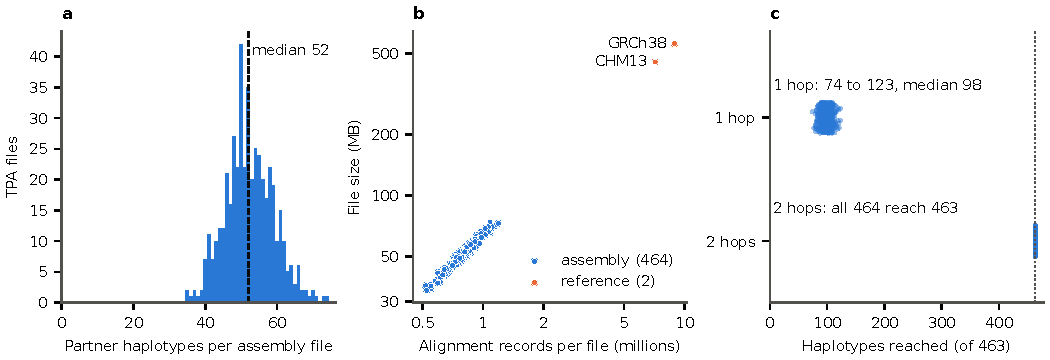
\includegraphics[width=\textwidth]{fig/fig2_release.pdf}
\caption{\label{fig:release}The HPRC r2 TPA files as an alignment network.
Each TPA file holds the alignments that target one haplotype, and its string table names every haplotype that the file aligns.
(\textbf{a}) Partner haplotypes per assembly file for the 464 assembly files.
Counts include GRCh38 and CHM13 where a file lists them (45 and 51 files).
The dashed line marks the median, 52.
The GRCh38 and CHM13 files list 465 partners each and are not shown.
(\textbf{b}) File size in the S3 listing against alignment records in the header, for all 466 files, on log axes.
The two reference files are labelled.
(\textbf{c}) Non-reference haplotypes reached from each of the 464 assembly haplotypes in the undirected pair graph without GRCh38 and CHM13.
One hop counts direct partners stored in either file, and two hops add their partners.
The dotted line marks all 463 others, and points are spread vertically for visibility.
Pairs come from sequence names, not from aligned bases, and E3 measures reach in bases.
Data are the 466 string tables and the S3 listing in data/, and the script is scripts/fig2\_release.py.}
% src: scripts/fig2_release.py stdout (panel a histogram, panel b ranges, panel c histograms); data/pairs_out.txt; data/partner_summary.txt
\end{figure*}
